\documentclass[12pt]{article}
\usepackage[catalan]{babel}
\usepackage[utf8]{inputenc}
\usepackage{graphicx}
\usepackage{lscape}

\begin{document}
\begin{titlepage}
		\centering
		
\includegraphics[width=0.7\textwidth]{imatges/icona_gran.png}\par\vspace{1cm}
		{\huge\bfseries IT-EXAMS\par}
		\vspace{1cm}
		{\scshape\Large Pla d'empresa\par}
		\vspace{1cm}
		{\scshape\Large Màster en enginyeria informàtica\par}
		\vspace{1.5cm}
		{\Large\itshape Oscar Galera i Alfaro\par}
		\vfill
		{\large \today\par}
\end{titlepage}
\tableofcontents

\clearpage
\section{Resum executiu}
\clearpage
\section{Proposta de valor}
IT-Exams és una plataforma que permet accedir des de qualsevol dispositiu i plataforma a un motor d'exàmens relacionats amb el món de les noves tecnologies, d'una manera intuitiva, àgil i dinàmica. 
\\\\Aquesta eina utilitza les últimes versions d'exàmen distribuides per les empreses certificadores i compta amb més de 690 examens de més de 50 empreses reconegudes en el sector, tals com Google, Amazon, Oracle o Linux per nombrar-ne algunes. 
\\\\És ideal per complementar altre material d'estudi com ara llibres o material en línia i està pensada per totes aquelles persones que vulguin ampliar els seus coneixements, i fer-se més competitius en l'àmbit laboral, obtenint una certificació que acrediti a nivell mundial els seus coneixements tècnics. 
\\\\Aquesta eina però, també pot utilitzar-se per recolçar el material impartit en cursos de preparació o per evaluar el coneixement tècnic dels treballadors del departament de noves tecnologies de tot tipus d'empreses petites, mitjanes i grans.
\\\\A diferència d'altres eines amb propòsits similars, aquesta plataforma dóna un ampli ventall d'opcions i preus que s'adapten a totes les necessitats de qualsevol usuari.
\begin{landscape}
\begin{figure}
	\centering
	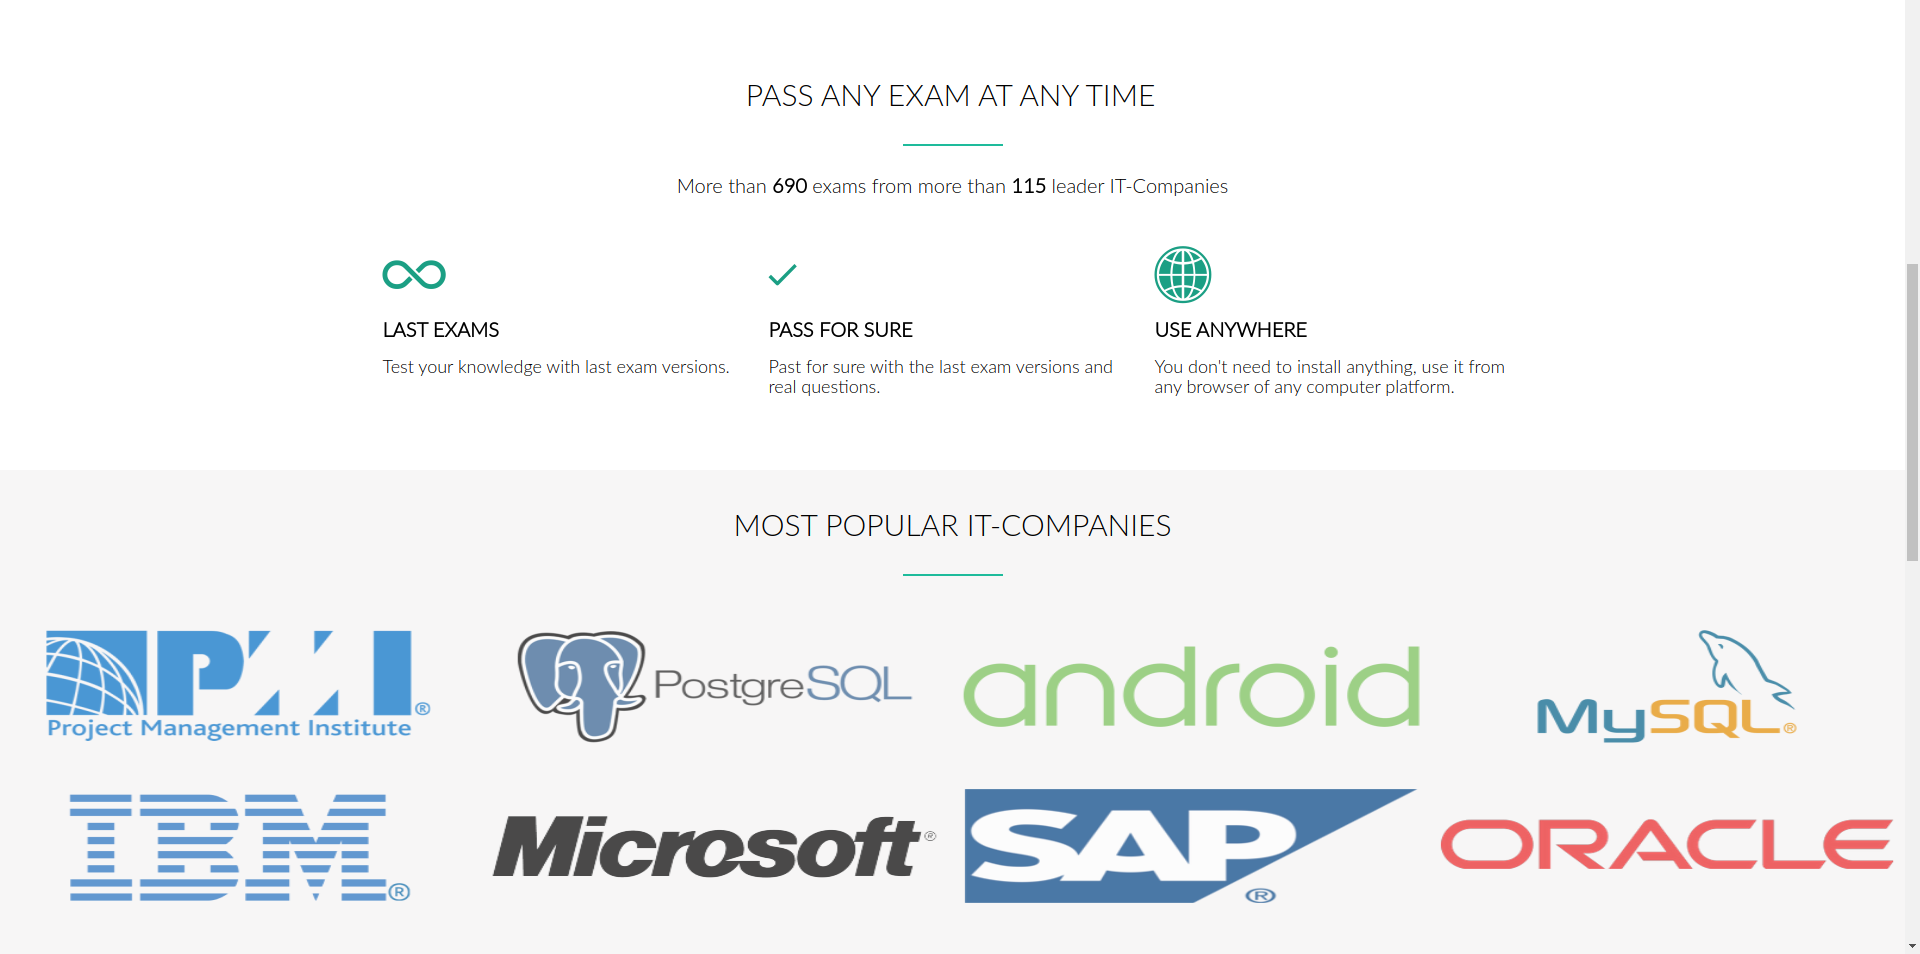
\includegraphics[width=1.5\textwidth]{imatges/valor.png}\par\vspace{1cm}
	\caption{Sumat al canvi tecnologic i marca la diferència!}
\end{figure}
\end{landscape}
\subsection{Per què és important comptar amb una certificació IT alhora de buscar feina?}

\subsection{Model canvas}
En el següent diagrama es pot veure de forma 




\clearpage
\section{Servei}
El servei que preten donar l'empresa, és un servei web que compta amb les següents propietats.
\begin{itemize}
	\item \textbf{Robuts:} Estarà dissenyat per donar servei a una gran quantitat d'usuaris sense que es vegi afectat el rendiment.
	\item \textbf{Altament disponible:} Accesible les 24 hores, els 365 dies de l'any.
	\item \textbf{Portable:} Es podrà utilitzar en qualsevol dispositiu que utilitzi qualsevol navegador web.
	\item \textbf{Flexible:} Permetrà diverssos tipus d'accés i formes de treball adaptant-se a les diferents necessitats dels usuaris.
	\item \textbf{Segur:} Totes les dades sensibles es tractaràn de forma encriptada.
	\item \textbf{Intuitiu:} Els components del servei seràn el màxim sencills posibles per a que l'usuari pugui utilitzar-lo sense cap tipus de problema.
	\item \textbf{Amigable:} El disseny serà amigable per a que l'usuari tingui una bona experiencia.
	\item \textbf{Responsable:} S'adaptarà el servei per poder ser utilitzat per persones amb discapacitats.
	\item \textbf{Amb garanties:} Si l'usuari no supera la prova i pot acreditar-ho, s'ampliarà el temps d'ús del servei per a que pugui continuar treballant amb nosaltres.
\end{itemize} 




\clearpage
\section{Mercat}
El servei IT-EXAM està destinat a diferents sectors de mercat.
\subsection{Mercat disponible total (\textit{TAM})}
El mercat total que podem abastir amb el producte es descriu en les següents seccions.
\subsubsection{Persones físiques}
Aquest és el sector de mercat més important de l'empresa, abarca tots aquelles persones (joves i adults principalment) que volen obtenir una certificació IT per ampliar els seus coneixements i així millorar les seves condicions laborals i han decidit fer-ho de forma autònoma.
\\\\El perfil d'aquestes persones sol ser homes d'una edat entre 18 i 50 anys, amb ganes d'autosuperació i d'ampliar els seus coneixements, típicament per obtenir més oportunitats laborals.
\\\\El benefici que obté aquest sector del servei, és el fet de màximitzar el resultat dels esforços invertits en la preparació per una certificació.

\subsubsection{Empreses de preparació per a certificacions IT}
Després de l'alt increment en la demanda de certificacions IT en les empreses (especialment en l'àmbit privat). Moltes entitats certificadores van especialitzar-se en la preparació pels examens o van contractar terceres empreses especialitzades.
\\\\El perfil d'aquestes empreses, sol ser d'epresa petita/mitjana situades aprop de grans ciutats i que compten amb sistemes informàtics grans i un ampli material per preparar les classes presencials i en línia.
\\\\Aquest també és un sector important per l'empresa, degut a que necesiten serveis de qualitat per millorar els coneixements dels seus clients i nosaltres podem representar un proveidor important de continguts per a ells.
\\\\El benefici que obté aquest sector del servei, són els beneficis que aporten els clients de l'empresa que utilitza el servei.

\subsubsection{Empreses amb departament de noves tecnologies}
Totes les empreses d'avui dia (especialment les grans) acostumen a tenir un departament d'informàtica. En ocasions va bé mesurar els coneixements del personal per veure quin és l'equip òptim per dur a terme un nou projecte.
\\\\El perfil d'aquestes empreses que ens interesa especialment, és principalment el d'empresa mitjana/gran amb un departament de noves tecnologies que compta amb un personal amb molts anys d'experiència. Al qual podem aportar una font de coneixement i fer de 
\\\\En aquest àmbit, també ens interessa proporcionar la plataforma al departament de recursos humans per validar els coneixements dels nous treballadors tecnologics que han de començar a formar part de l'empresa.
\\\\El benefici que obté aquest sector del servei, es basa en millorar el talent del departament d'informàtica filtrant personal no preparat i d'aquesta manera, augmentar la productivitat de l'empresa.

\subsection{Mercat segmentat disponible (\textit{SAM})}
La intenció de l'empresa és arribar a els tres sectors destacats en el \textit{TAM}. Per aquest motiu, es considerem que tenim a nivell d'emrpesa un mercat disponible total igual al mercat segmentat disponible.

\subsection{Mercat compartit disponible (\textit{SOM})}
Durant els primers dos-tres anys, l'empresa es centrarà en el mercat de les persones físiques. Aquesta decisió s'ha pres tenint en compte que és el sector del mercat amb el qual és més fàcil iniciar-se. 
\\\\Pasats uns anys i amb l'experiencia i reconeixement obtingut per part dels clients, reconsiderarém noves metes, en les quals hi haurà les empreses especialitzades i empreses privades de tot tipus.
\begin{landscape}
\begin{figure}
	\centering
	
\includegraphics[width=0.5\textwidth]{imatges/icon.png}\par\vspace{1cm}
\end{figure}
\end{landscape}



\clearpage
\section{Competència}
La competència en el sector del suport per l'aprenentatge és molt rigurosa i hi ha moltes empreses que ofereixen productes similars. Per tal de analitzar quines aventatges té el servei que es vol oferir, he desenvolupat la següent matriu de competències on comparo el servei ofertat amb els serveis que es proporcionen en els portals web \textit{https://www.pass4sure.com} i \textit{http://www.testking.com/}.
\begin{landscape}
\begin{figure}
	\centering
	
\includegraphics[width=0.5\textwidth]{imatges/icon.png}\par\vspace{1cm}
\end{figure}
\end{landscape}
\clearpage



\section{Pla de venda}
\clearpage
\section{Mileston and metrics}
\clearpage
\section{Equip de gestió}
\clearpage
\section{Pla financer}
\clearpage
\appendix
\end{document}